\documentclass[a4paper]{article}

\usepackage{/home/evasilyev/CLionProjects/algorithmic_foundation/settings}


\begin{document}

Given a reference of a node in a connected undirected graph. Return a deep copy (clone) of the graph. Each node in the graph contains a val (int) and a list (List[Node]) of its neighbors.

\begin{lstlisting}[style=C++]
/*
// Definition for a Node.
class Node {
public:
    int val;
    vector<Node*> neighbors;
    
    Node() {
        val = 0;
        neighbors = vector<Node*>();
    }
    
    Node(int _val) {
        val = _val;
        neighbors = vector<Node*>();
    }
    
    Node(int _val, vector<Node*> _neighbors) {
        val = _val;
        neighbors = _neighbors;
    }
};
*/
\end{lstlisting}

\textbf{Test case format:}

For simplicity sake, each node's value is the same as the node's index (1-indexed). For example, the first node with $val = 1$, the second node with $val = 2$, and so on. The graph is represented in the test case using an adjacency list.

Adjacency list is a collection of unordered lists used to represent a finite graph. Each list describes the set of neighbors of a node in the graph.

The given node will always be the first node with $val = 1$. You must return the copy of the given node as a reference to the cloned graph.

\SPACE

\textbf{Example 1:}

\begin{center}
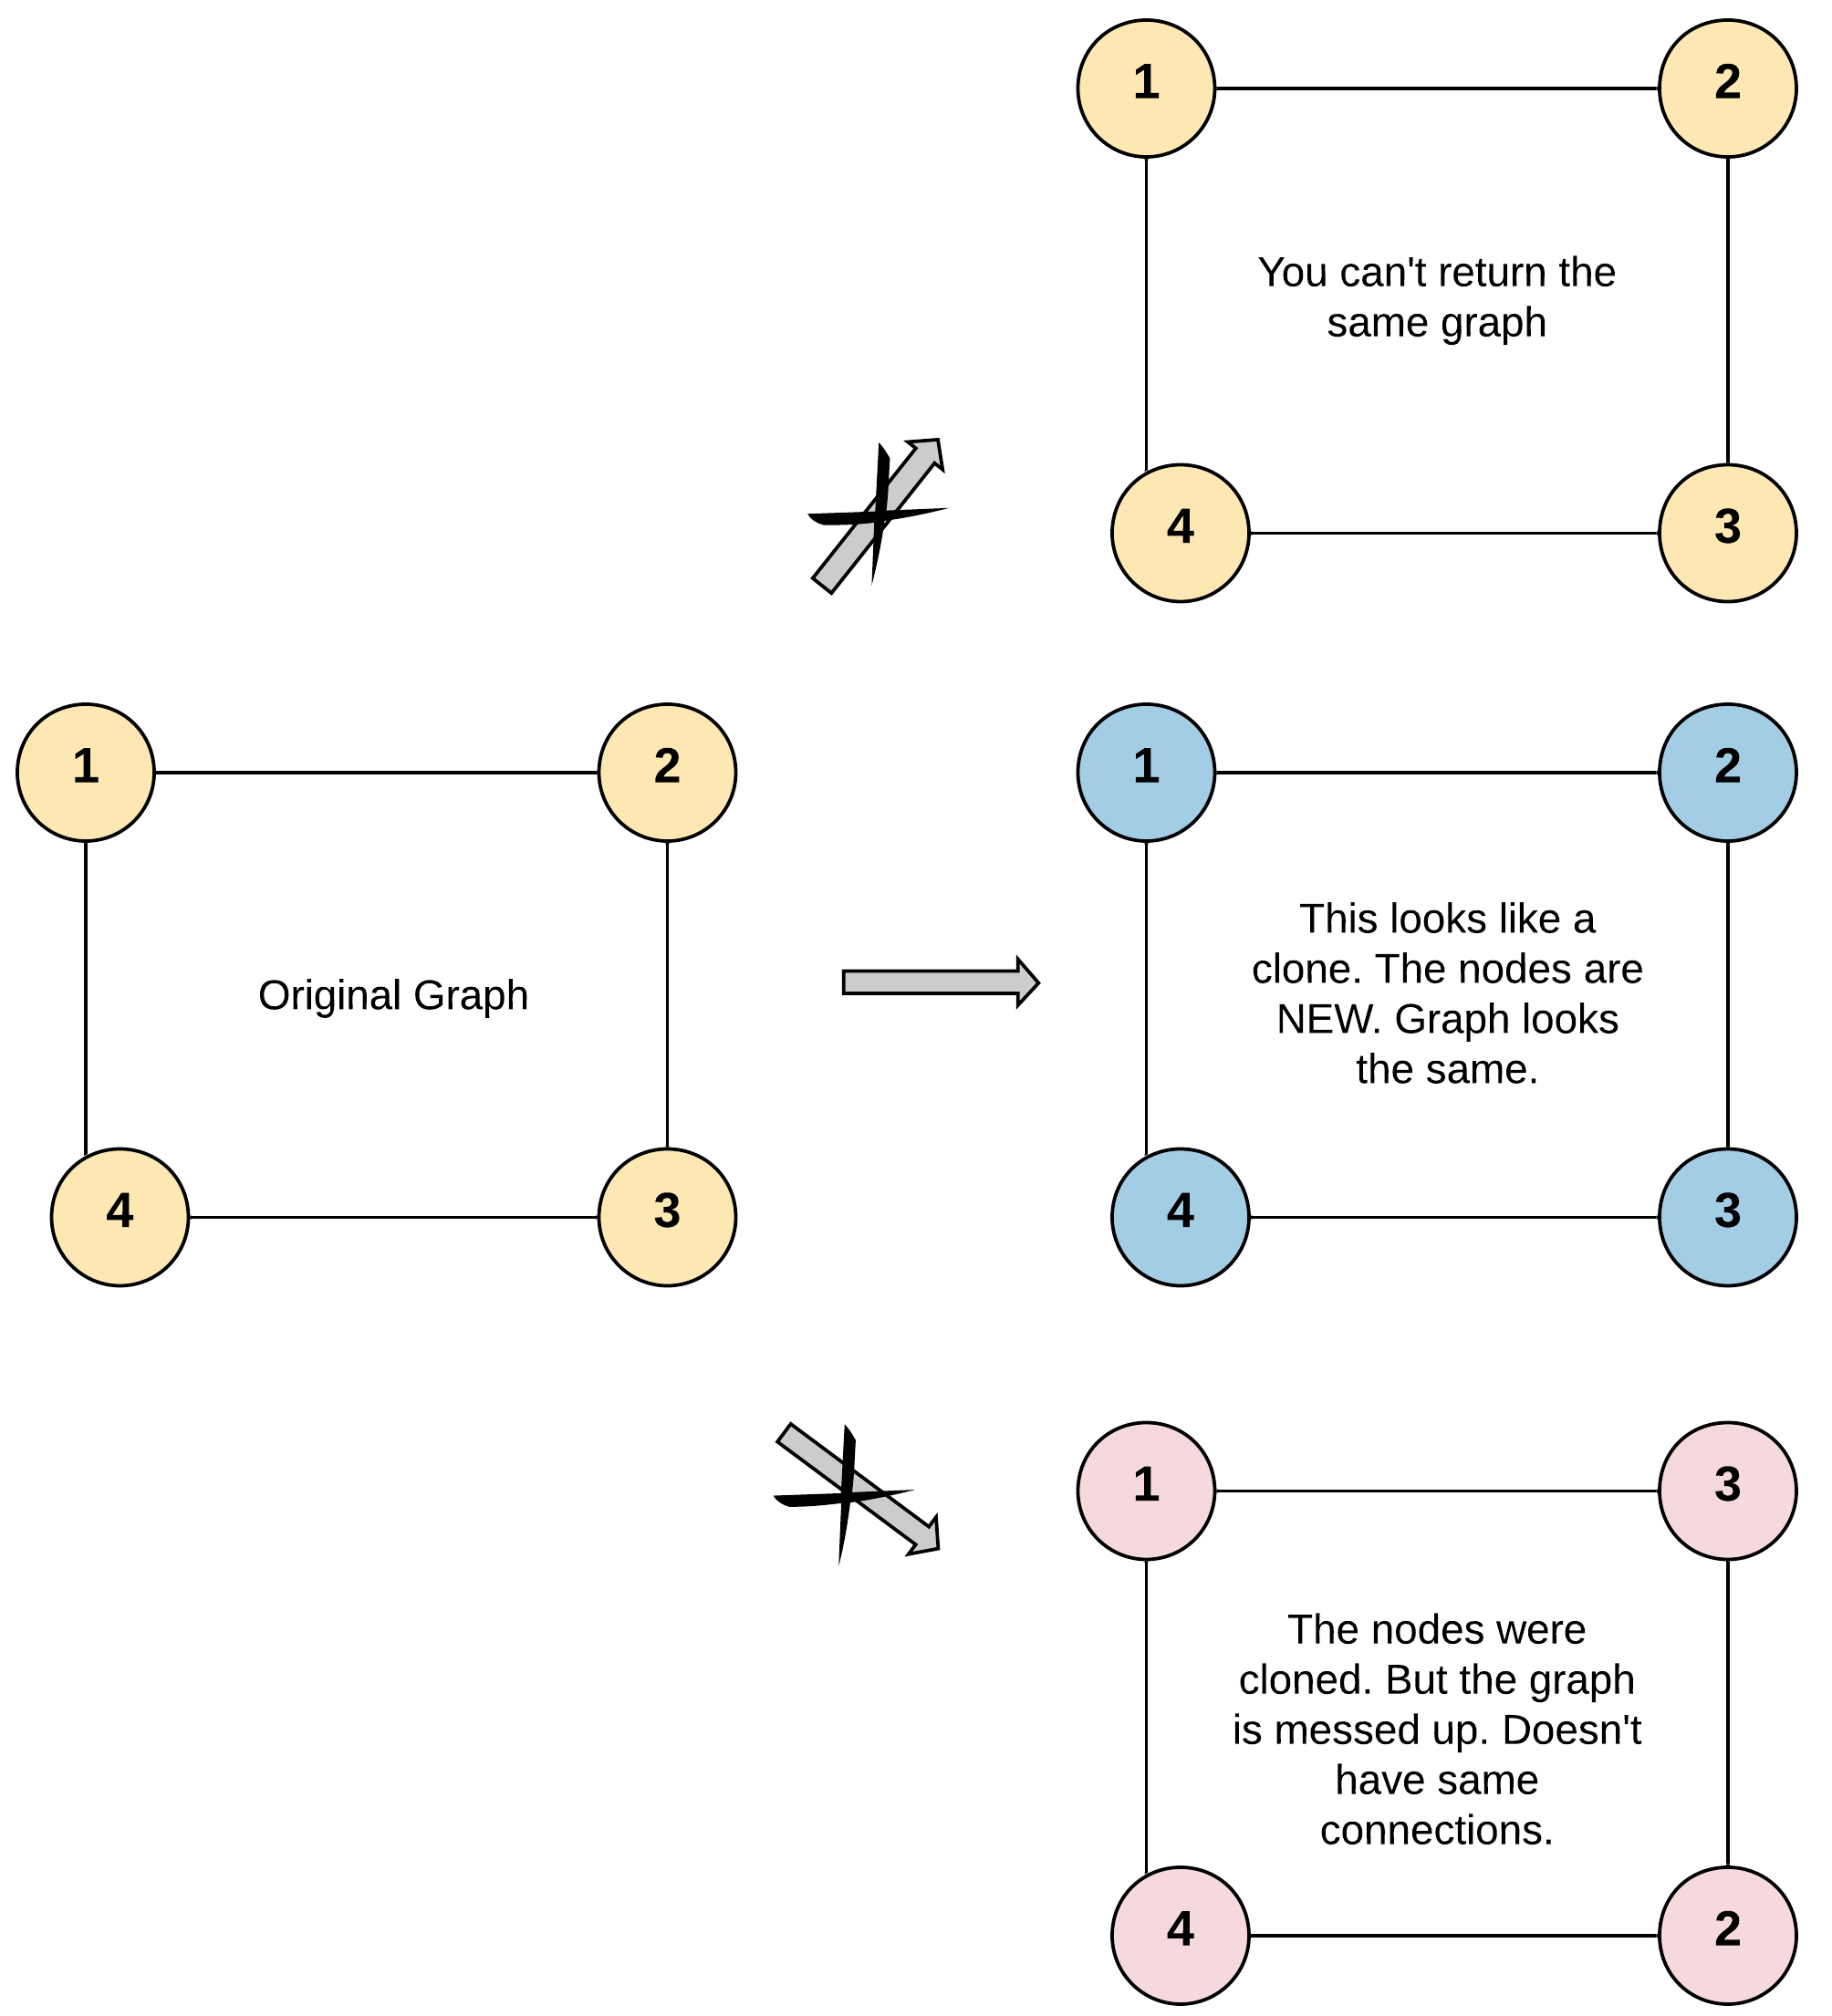
\includegraphics[width=10cm]{images/1.png}
\end{center}

\textbf{Input:} adjList = [[2,4],[1,3],[2,4],[1,3]]

\textbf{Output:} [[2,4],[1,3],[2,4],[1,3]]

\textbf{Explanation:} There are 4 nodes in the graph.\\
1st node ($val = 1$)'s neighbors are 2nd node ($val = 2$) and 4th node ($val = 4$).\\
2nd node ($val = 2$)'s neighbors are 1st node ($val = 1$) and 3rd node ($val = 3$).\\
3rd node ($val = 3$)'s neighbors are 2nd node ($val = 2$) and 4th node ($val = 4$).\\
4th node ($val = 4$)'s neighbors are 1st node ($val = 1$) and 3rd node ($val = 3$).


\SPACE


\textbf{Example 2:}
\begin{center}
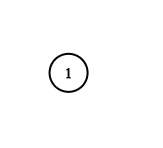
\includegraphics[width=4cm]{images/2.png}
\end{center}

\textbf{Input:} adjList = [[]]

\textbf{Output:} [[]]

\textbf{Explanation:} Note that the input contains one empty list. The graph consists of only one node with $val = 1$ and it does not have any neighbors.


\SPACE


\textbf{Example 3:}

\textbf{Input:} adjList = []

\textbf{Output:} []

\textbf{Explanation:} This an empty graph, it does not have any nodes.


\SPACE

\textbf{Example 4:}
\begin{center}
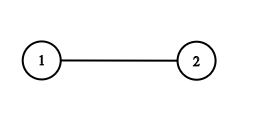
\includegraphics[width=8cm]{images/3.png}
\end{center}

\textbf{Input:} adjList = [[2],[1]]

\textbf{Output:} [[2],[1]]


\SPACE

\textbf{Constraints:}

\begin{itemize}
\item $1 \le Node.val \le 100$
\item $Node.val$ is unique for each node
\item Number of Nodes will not exceed $100$
\item There is no repeated edges and no self-loops in the graph
\item The Graph is connected and all nodes can be visited starting from the given node
\end{itemize}








\end{document}
